\documentclass[10pt]{article}
\usepackage{ctex}
\usepackage{graphicx}
\graphicspath{{E:/大学课程/大一下/人工智能程序设计/作业集/第九周作业/},{pics/}}
\usepackage{amsmath}
\usepackage{amssymb}
\usepackage{float}%使图片紧跟在文字后面

\title{第九周问答作业}
\author{朱士杭\ 231300027}
\date{\kaishu \today}

\begin{document}
	\maketitle
	\section{问题一:科里化及其应用场景}
	\subsection{什么是科里化}
科里化(Currying)是一种在函数式编程中常用的技巧,它将一个接受多个参数的函数转换为一系列使用一个参数的函数。\par
更具体地说,科里化是将一个 n 元函数转换成 n 个一元函数的过程。
每个一元函数返回一个新的一元函数,直到所有参数都被应用。
在科里化过程中,我们不是一次性传递所有参数,而是每次传递一个参数,并且返回一个新的函数,这个新函数等待下一个参数。
这个过程一直重复,直到所有参数都传递完毕。
\subsection{科里化使用场景}
参数复用:当我们需要多次调用某个函数,并且这个函数的大部分参数在每次调用中都是相同的,可以使用科里化来避免重复传递这些参数。\par
函数组合:在函数式编程中,科里化使得函数组合变得更加容易,因为科里化后的函数总是返回一个新函数,这与其他函数的输出可以很容易地结合起来。\par
动态函数创建:科里化允许我们创建新的函数,这些函数预设了一些参数,这在需要根据特定条件动态生成函数时非常有用。\par
延迟计算:当我们不想立即执行一个函数,而是想要在未来的某个时间点执行时,科里化可以帮助我们“记住”已经提供的参数,并在需要时应用剩余的参数。\par
 优化代码:在某些情况下,科里化可以用来优化代码的结构,使其更加模块化和可维护。
\section{问题二:map函数的功能及其用途}
\subsection{map函数功能}
它用于将一个函数应用于一个序列(如列表、元组或字符串)中的每个元素,并返回一个迭代器,其中包含应用函数后的结果。\par
简单来说,map用于对序列中的每个元素执行同一个操作,就跟map的名字一样,本身就是一种映射关系,甚至于说是一种双射。\par
\subsection{map函数用途}
批量处理数据:当你需要对一个数据集合中的每个元素执行相同的操作时,map非常有用。
例如,如果你有一个数字列表,并想要将每个数字乘以2,可以使用map来实现。\par
函数式编程:在函数式编程中,map是一个基本的概念,它允许你将函数作为第一个类对象(first-class citizen)来处理,即将函数作为参数传递给其他函数。\par
代码简洁:使用map可以使得代码更加简洁,尤其是当你需要对多个序列进行相同的操作时。
map可以接受多个序列作为输入,只要函数接受多个参数即可。\par
性能优化:在某些情况下,使用map可以比传统的循环方法更高效,尤其是在处理大规模数据时(好像是因为分布式处理的缘故吧)
\section{复合函数概念及其用途}
\subsection{复合函数概念}
python中的函数复合概念和数学中的函数复合相当类似,如果将函数视为一种运算的话,由于运算具有顺序,函数结合也是由顺序的,
但是将不同函数作用视为一个整体的话记为函数复合,将一个函数的输出作为另一个函数的输入,从而创建一个新的函数。
\subsection{复合函数用途}
代码重用和模块化:通过组合现有的函数,你可以创建新的函数而无需编写全新的代码。这有助于代码重用并促进模块化设计。\par
简化复杂操作:函数复合允许你将复杂的操作分解为更小、更简单的函数。然后,你可以将这些简单函数组合起来,以执行更复杂的任务。并且在函数式编程当中,它允许你以声明式的方式描述数据处理流程,而不是以命令式的方式。\par
提高代码可读性:通过组合函数,你可以创建一个清晰的操作链,这有助于提高代码的可读性和可维护性。

\section{抽象与封装}
关于抽象其实分为过程抽象与数据抽象,过程抽象主要针对于函数式编程,而数据抽象主要针对面向对象编程\par
抽象允许我们创建模型,这些模型只包含对解决问题至关重要的特征,而忽略不必要的细节,仅用一个名字就完成了一个过程或者一个对象\par
封装是指将数据(属性)和操作数据的方法(函数)捆绑在一起,形成一个统一的单元,即对象。\par
封装的目的是隐藏对象的内部状态和实现细节,只暴露必要的接口与外部通信。
这样,对象的内部表示就不能被外部直接访问和修改,必须通过定义好的接口进行。\par
封装实际上类似于一种黑盒的存在,在程序中将过程与数据打包并且对外部不可见,从而实现保护数据隐私以及过程隐蔽性\par
在python当中抽象和封装主要通过类来实现,通过创建一个类对应的实例即对象来生成一块独立的个体,在这个个体里面可以定义成员函数来实现过程抽象,可以设置对象专属的数据来实现数据抽象与封装


\section{面向对象与面向过程程序设计}
面向对象程序设计是一种以对象为基础的编程范式,它将数据和操作数据的方法封装在一起,形成对象。\par
OOP(Object-Oriented-Program)的核心理念是将现实世界的实体抽象为程序中的对象,并通过对象之间的交互来完成任务。\par
基于过程的程序设计是一种以过程(函数或方法)为中心的编程范式。\par
在过程式编程中,程序被划分为一系列的函数,这些函数按照一定的顺序执行,以完成特定的任务。
过程式编程关注的是函数和程序流程,而不是数据和对象\par

面向对象程序设计有哪些基本特征嘞:抽象、封装、继承、多态(这个在上个学期的C++里面已经讲过啦太经典的问题啦哈哈哈)


\section{make\_filter高阶函数}
\begin{figure}[H]
	\centering
	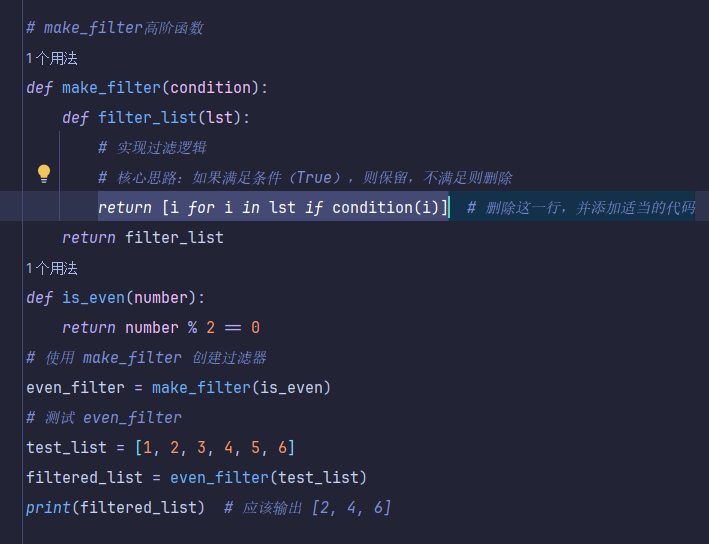
\includegraphics[scale=0.9]{过滤器}
	\caption{使用高阶函数创建过滤器}
\end{figure}
在这里核心思路就是创建高阶函数make\_filter,并且在内部定义一个过滤函数并将其返回,到时候只需要判断是否满足条件condition即可,这里return很简单,使用一下最基本的列表解析即可如果满足则包含在列表当中,不满足则丢掉即可


\section{Book类模拟图书借阅过程}
\begin{figure}[H]
	\centering
	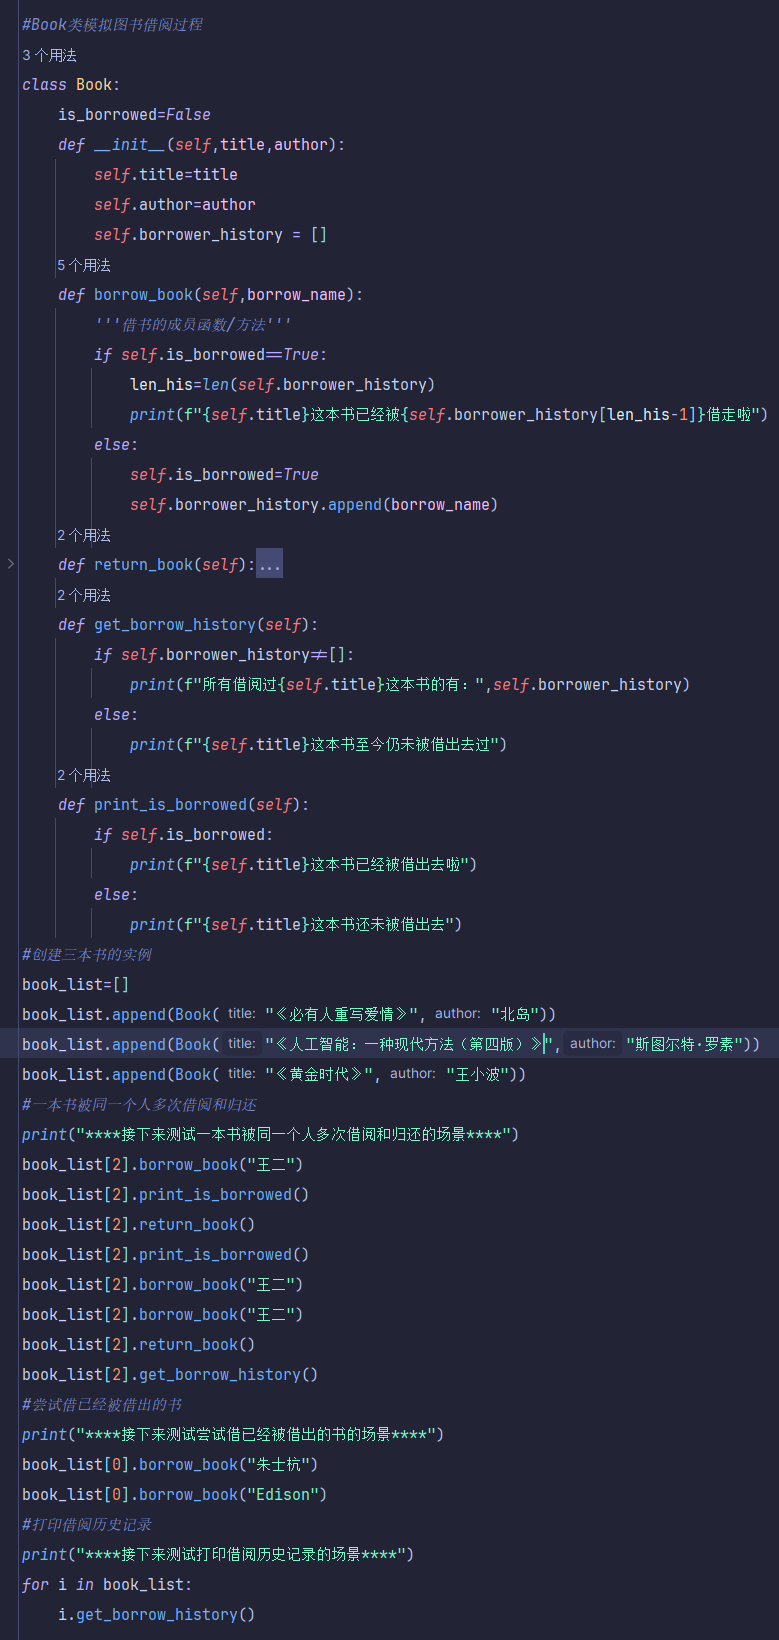
\includegraphics[scale=0.5]{图书馆}
	\caption{模拟图书借阅过程}
\end{figure}
\begin{figure}[H]
	\centering
	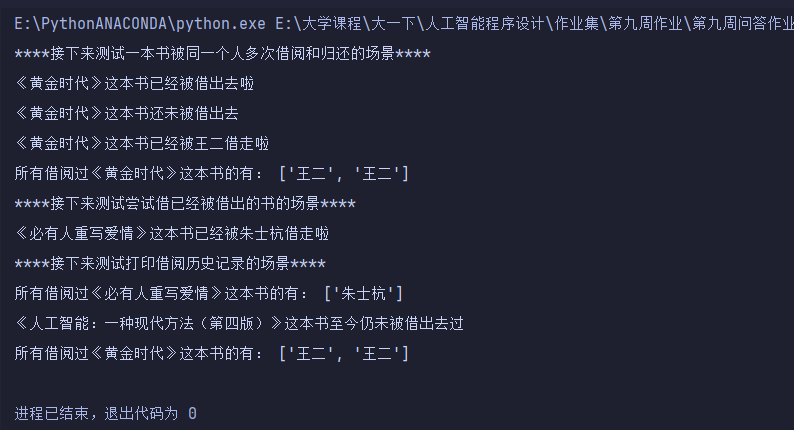
\includegraphics[scale=0.8]{运行结果}
	\caption{代码运行结果}
\end{figure}

\end{document}